\documentclass[a4paper,11pt]{jsarticle}
\usepackage{graphicx}
\usepackage{wrapfig}
\usepackage{amsmath,amssymb,amsthm}
\usepackage{amssymb}
\usepackage{ascmac}
\usepackage{subfigure}
\usepackage{bm}
\usepackage{setspace}
\usepackage{cases}%左かっこつけるときに必要だった
\usepackage{leftidx}%行列表示用?
\usepackage{fancyhdr}
\usepackage{graphicx}
\usepackage{float}
\usepackage{booktabs}
\usepackage{url}
\usepackage{bm}
\usepackage{verbatim}
\usepackage{calc} 

\setlength{\headsep}{5mm}
\setlength{\oddsidemargin}{-0.5zw} %→にズラす
\setlength{\textheight}{37\baselineskip}
\addtolength{\textheight}{\topskip}
\setlength{\topmargin}{-10mm}
\setlength{\textwidth}{45zw} %文章の幅
\setlength{\textheight}{215mm}
\setlength{\parindent}{1zw}%箇条書きの一文字下げ
\pagestyle{fancy}

\newtheorem{theorem}{定理}
\newtheorem{prop}[theorem]{命題}
\newtheorem{lemma}[theorem]{補題}
\newtheorem{cor}[theorem]{系}
\newtheorem{example}[theorem]{例}
\newtheorem{definition}[theorem]{定義}
\newtheorem{rem}[theorem]{注意}
\newtheorem{guide}[theorem]{参考}
\renewcommand{\proofname}{証明}

\numberwithin{theorem}{section}  % 定理番号を「定理2.3」のように印刷
\numberwithin{equation}{section} % 式番号を「(3.5)」のように印刷
\newcommand{\argmax}{\mathop{\rm arg~max\,}\limits}
\newcommand{\argmin}{\mathop{\rm arg~min\,}\limits}
\newcommand{\st}{\mathop{\rm subject~to\,}\limits}
\newcommand{\sign}{\mathop{\rm sign\,}\limits}

\newcommand{\dom}{\mathop{\mathrm{\bf dom}}\nolimits}
\newcommand{\minimize}{\mathop{\mathrm{\rm minimize}}\limits}
\newcommand{\maximize}{\mathop{\mathrm{\rm maximize}}\limits}

\lhead{2012年度・CG最終レポート}
\chead{}
\rhead{12M42340}
\lfoot{チョウ シホウ}
\cfoot{\thepage}
\rfoot{6月11日}
\renewcommand{\footrulewidth}{0.4pt}
\title{2012年度・CG最終レポート}
\author{12M42340 チョウ シホウ}


\begin{document}
\pagenumbering{roman}
%\tableofcontents
%\cleardoublepage
\pagenumbering{arabic}
\renewcommand{\thepart}{\arabic{part}}

%\thispagestyle{empty}

\begin{itembox}[l]{問題1:Texturing}
\begin{enumerate}
\item
Explain {\bf aliasing} artifact of texturing from the point of view of the sampling theorem. This explanation must
have two parts. The first one is a description of the theoretical reason behind of the aliasing with equations and
illustrations. The second one is an experimental description base on the actual artifacts occurring while the animation
by the program, using snapshots of the animation.
\item Explain one texturing algorithm to avoid the artifact.
\end{enumerate}
\end{itembox}
Sourcecode:{\bf CG\_Final\_Code/MipMapping}

\begin{enumerate}
\item
{\bf aliasing(エイリアシング)}とは,信号をサンプリングを行う際,入力信号に含まれる周波数成分がサンプリング周波数の$\frac{1}{2}$よりも高い場合に生じる折り返し歪みの現象である.例えば,我々がレンガの壁などの模様が複雑な物体をピクセルの少ない画像にするときに,モアレ(干渉縞)が生じる現象もaliasingの一種である.今回のソースコードでは,$512\times 512$の{\bf DotImage}を$320\times320$以下にする時は,次の画像のようなaliasing現象が見られる.

\begin{figure}[H]
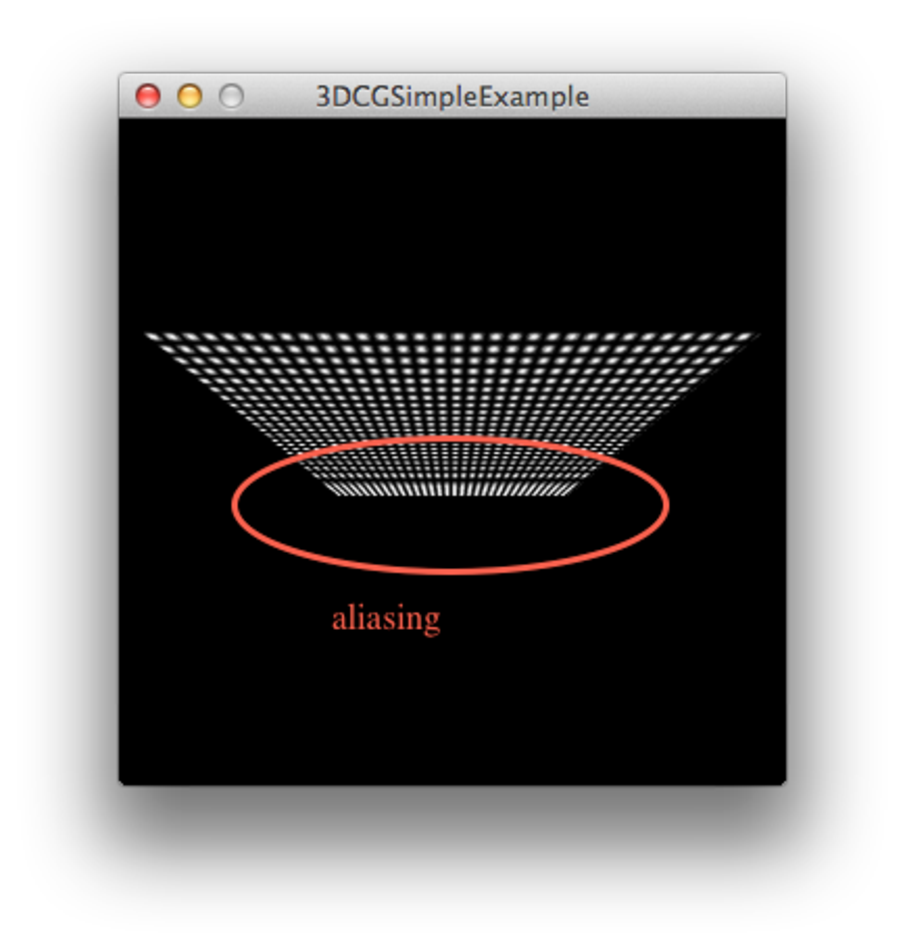
\includegraphics[bb=0 0 444 451,width=12.5cm]{with_out_mipmapping.pdf}
\end{figure}

\item 
aliasingが生じる原因は,信号の高周波成分に対し,サンプリング周波数がそのナイキスト条件(サンプリング周波数$f_s$と入力周波数$f_{\text{input}}$の関係は$f_s > 2f_{\text{input}}$)に満たさないこと.その場合,サンプリングを用いて高周波成分を再生する時に低周波のaliasing noiseになってしまう.例えば,次の画像のように,周波数が違う赤い正弦曲線と青い正弦曲線はサンプリング化によって全く同じ標本列を生成した.そのサンプリングは青い正弦曲線を再生できるが,赤い正弦曲線を再生できない.

aliasingを防ぐため,anti-aliasing技術がある.一般的には,サンプリングする前に,低周波成分をそのままで,高周波成分を低周波成分に近似し,低周波として再生される.

\begin{figure}[H]
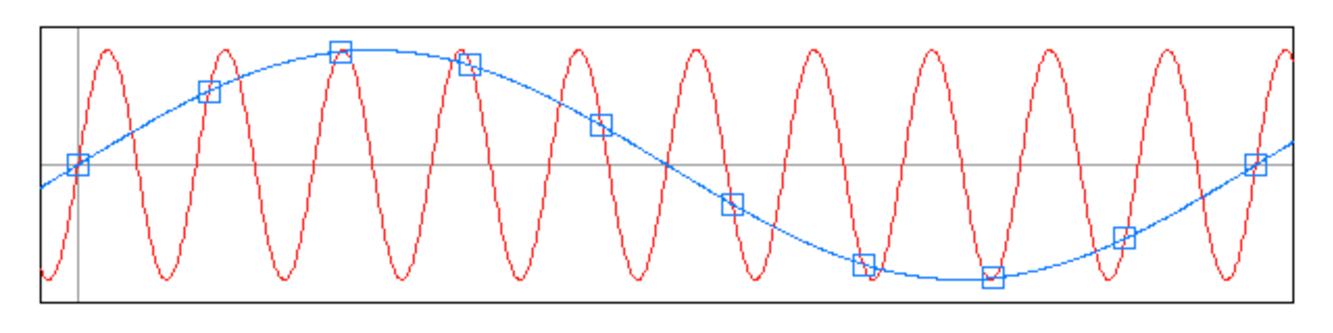
\includegraphics[bb=0 0 444 200,width=10.5cm]{Aliasing-plot.png}
\end{figure}

\item

CGにおける,代表的なanti-aliasingアルゴリズムはMipmappingである.Mipmapとは,3DCGにおいて,テクスチャ画像を補完する前に最適化された画像群である.この手法は描写速度を向上するだけではなく,aliasing現象も防げる.

Mipmappingのアルゴリズムは簡単である.メインのテクスチャの画像をあらかじめ処理し,複数のサイズに圧縮する.視点が近く場合,メインテクスチャを用いる,一方,遠くの視点に対し,圧縮されたMipmapを使う.例えば,$512\times512$のメインテクスチャには,サイズがそれぞれ$256\times256,128\times128,64\times64\dots$の画像群を生成し,レンダリング領域の大きさによって近似するMipmapを使えばよい,例としてレンダリング領域が$300\times300$の場合,$256\times256$と$128\times 128$の二枚のMipmapの$300\times300$となる線形結合を構造できる.

また,Mipmappingを使うと,テクスチャのサンプリングは視点の位置に関わらず必ずナイキスト条件を満たすため,aliasingに対する有効な解決手段と考えられる.

しかし,生成されたMipmapを保存するため,元のテクスチャの四倍の記憶領域が必要となるデメリットがある.
\begin{figure}[H]
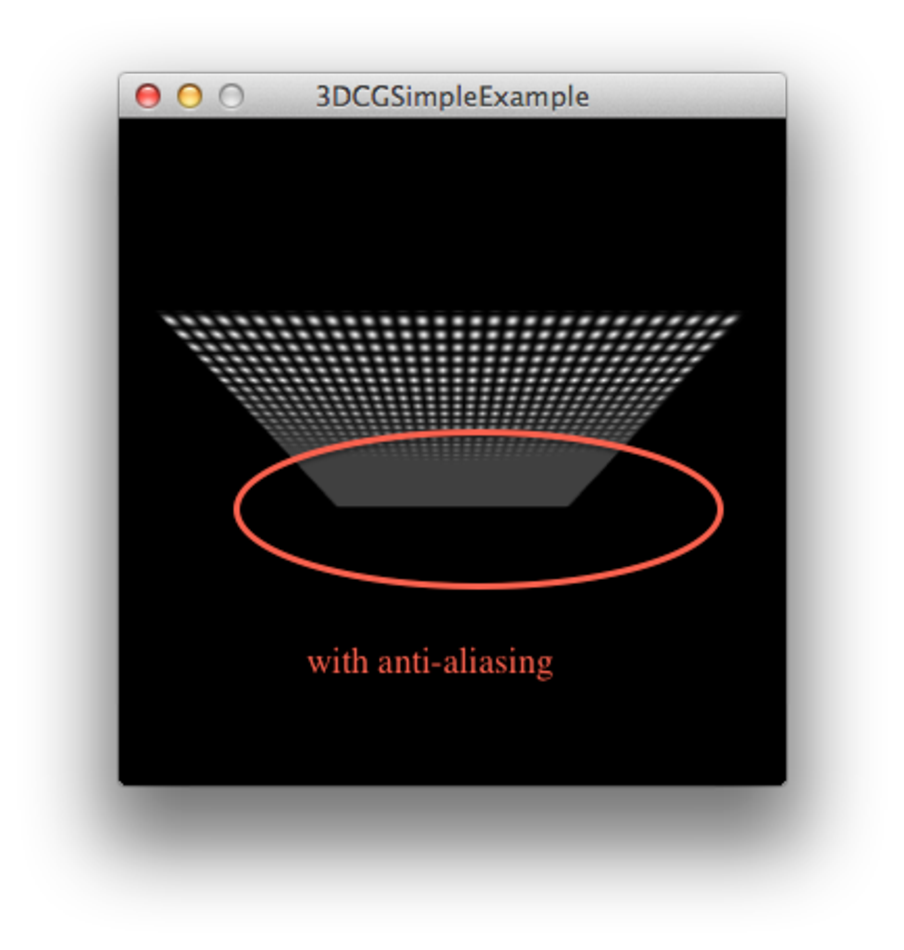
\includegraphics[bb=0 0 444 451,width=10.5cm]{with_mipmapping.pdf}
\end{figure}

一般的なテクスチャに対するも効果がある.

\begin{figure}[H]
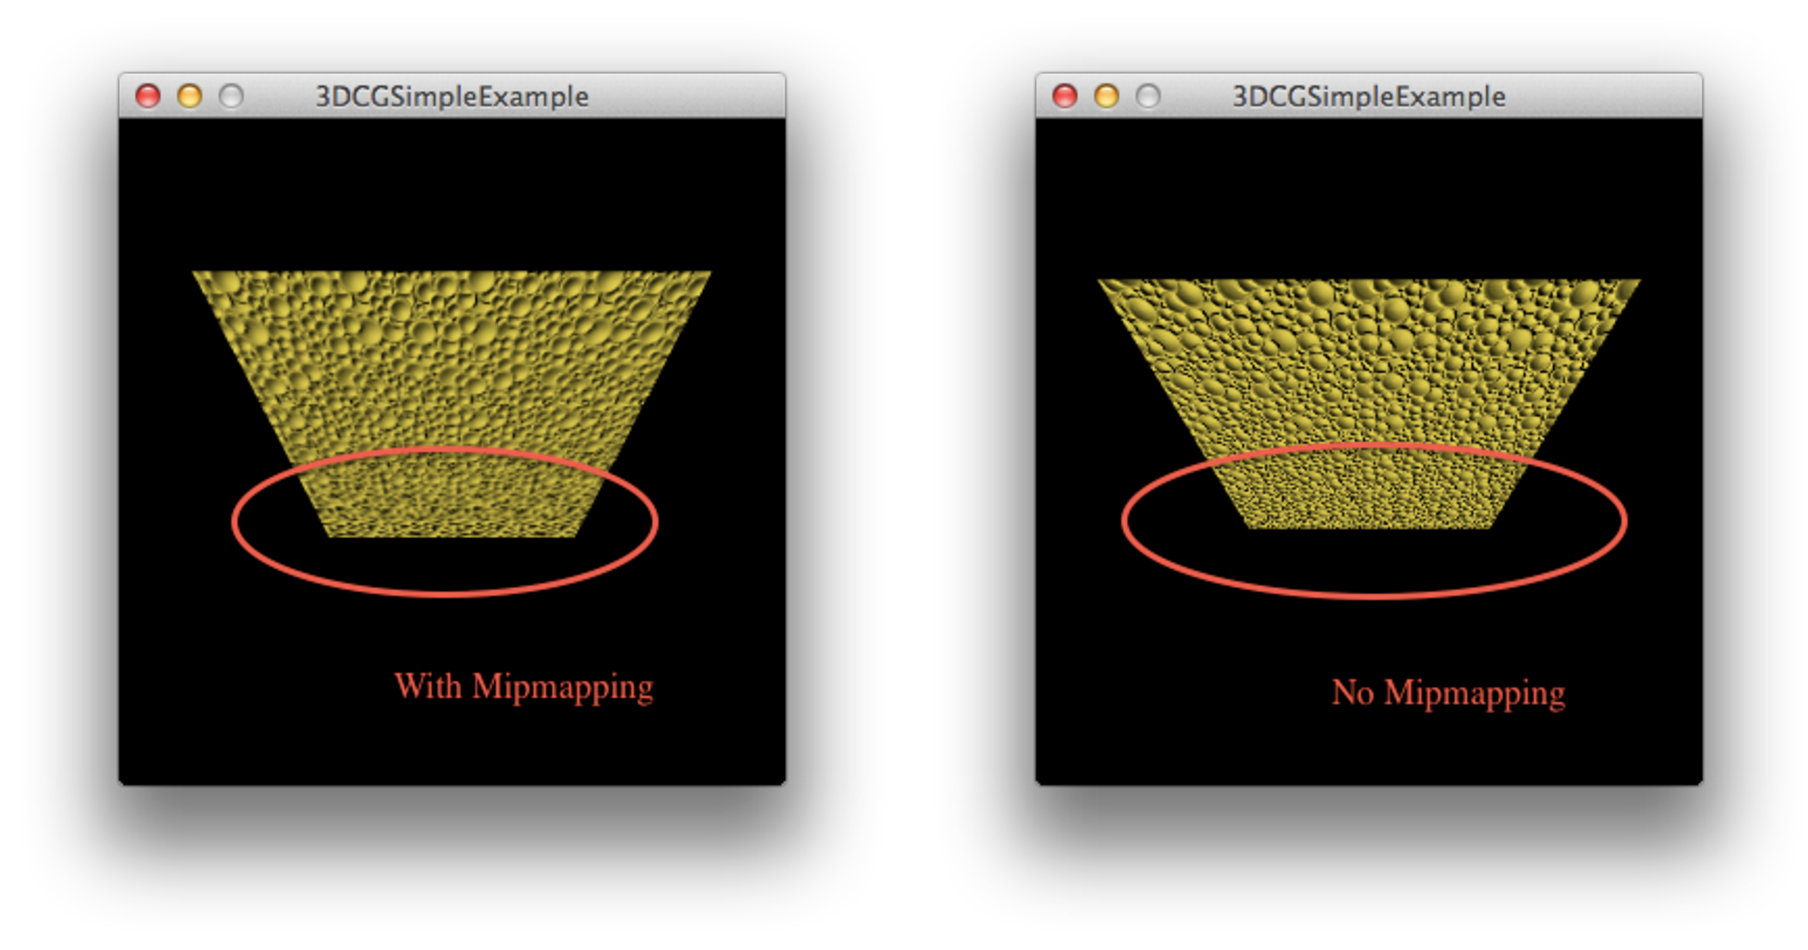
\includegraphics[bb=0 0 444 451,width=7.5cm]{mip_mapping.pdf}
\end{figure}



\end{enumerate}
\newpage

\begin{itembox}[l]{問題2:Geometry Data Definition and Transform}

Define a regular icosahedron whose center is the origin and whose one edge length is $0.8$, translate the center to
$(0,0,-2)$, and make an animation that it rotates around the vertical axis which passes through the center.

Use the same framework of the program and replace the plane to the icosahedron.

Put one snapshot on your report and describe how to compile and execute your program.
\end{itembox}

Sourcecode:{\bf CG\_Final\_Code/IcosahedronNormal}(Window sizeを二倍に拡大した)

Screenshot:
\begin{figure}[H]
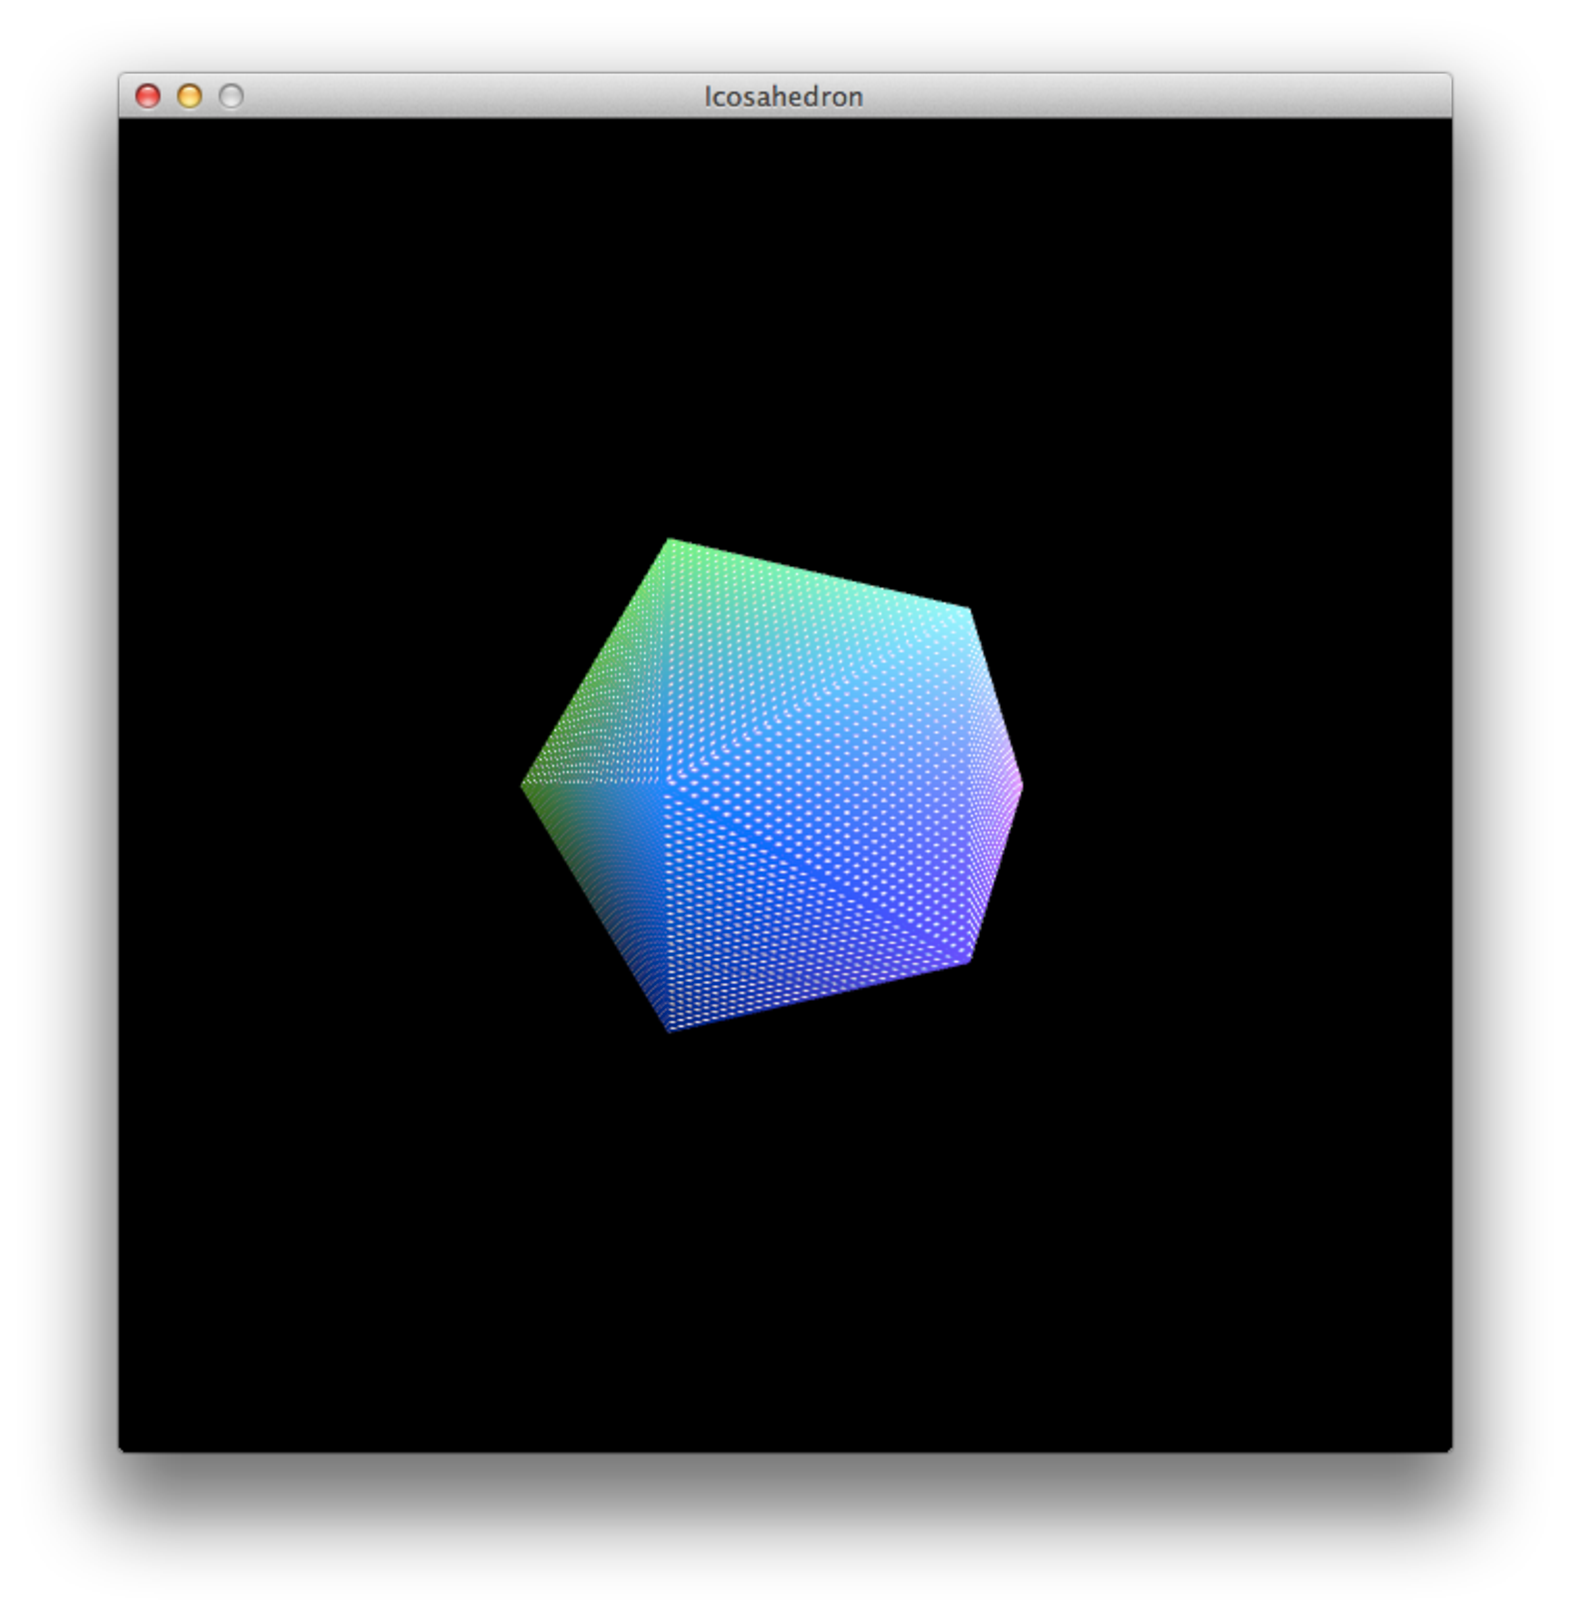
\includegraphics[bb=0 0 444 751,width=6cm]{Icosahedron.pdf}\\
\end{figure}

Wikipediaにより,辺の長さが$a$の二十面体の12個の頂点の座標は
\[
\frac{(0,\pm 1,\pm \phi)}{2}a,\frac{(\pm 1, \pm \phi,0)}{2}a,\frac{(\pm \phi, 0, \pm 1)}{2}a
\]
ただし,$\phi = \frac{1+\sqrt{5}}{2}$.また,二十面体のすべての面は面積が$\frac{\sqrt{3}}{4}a^2$となる正三角形である.例の{\bf Plane}の頂点と面の配置を上記に修正すれば二十面体になる.

\newpage

\begin{itembox}[l]{問題3:Reflection}
Calculate diffuse and ambient intensities on the surface of the regular icosahedron,as if it was a sphere,in the fragment shader stage.The equation to calculate the intensities $R_{\text{rgb}}$ is defined as
\[
R_{\text{rgb}} = C_{\text{rgb}}\Bigr( \max ( - \frac{LN}{|L||N|} ) + a \Bigr)
\]
where $C_{\text{rgb}}$ is the color of
the icosahedron, $N$ is the normal vector at a point, $L$ is the vector of an incident light direction and $a$ is a coefficient of
ambient light.

Set $L$ as an efficient direction to express shading effect on the object surface.



Put one snapshot on your report and describe how to compile and execute your program.
\end{itembox}

Sourcecode:{\bf CG\_Final\_Code/IcosahedronWithReflection}(Window sizeを二倍に拡大した)

Screenshot:
\begin{figure}[H]
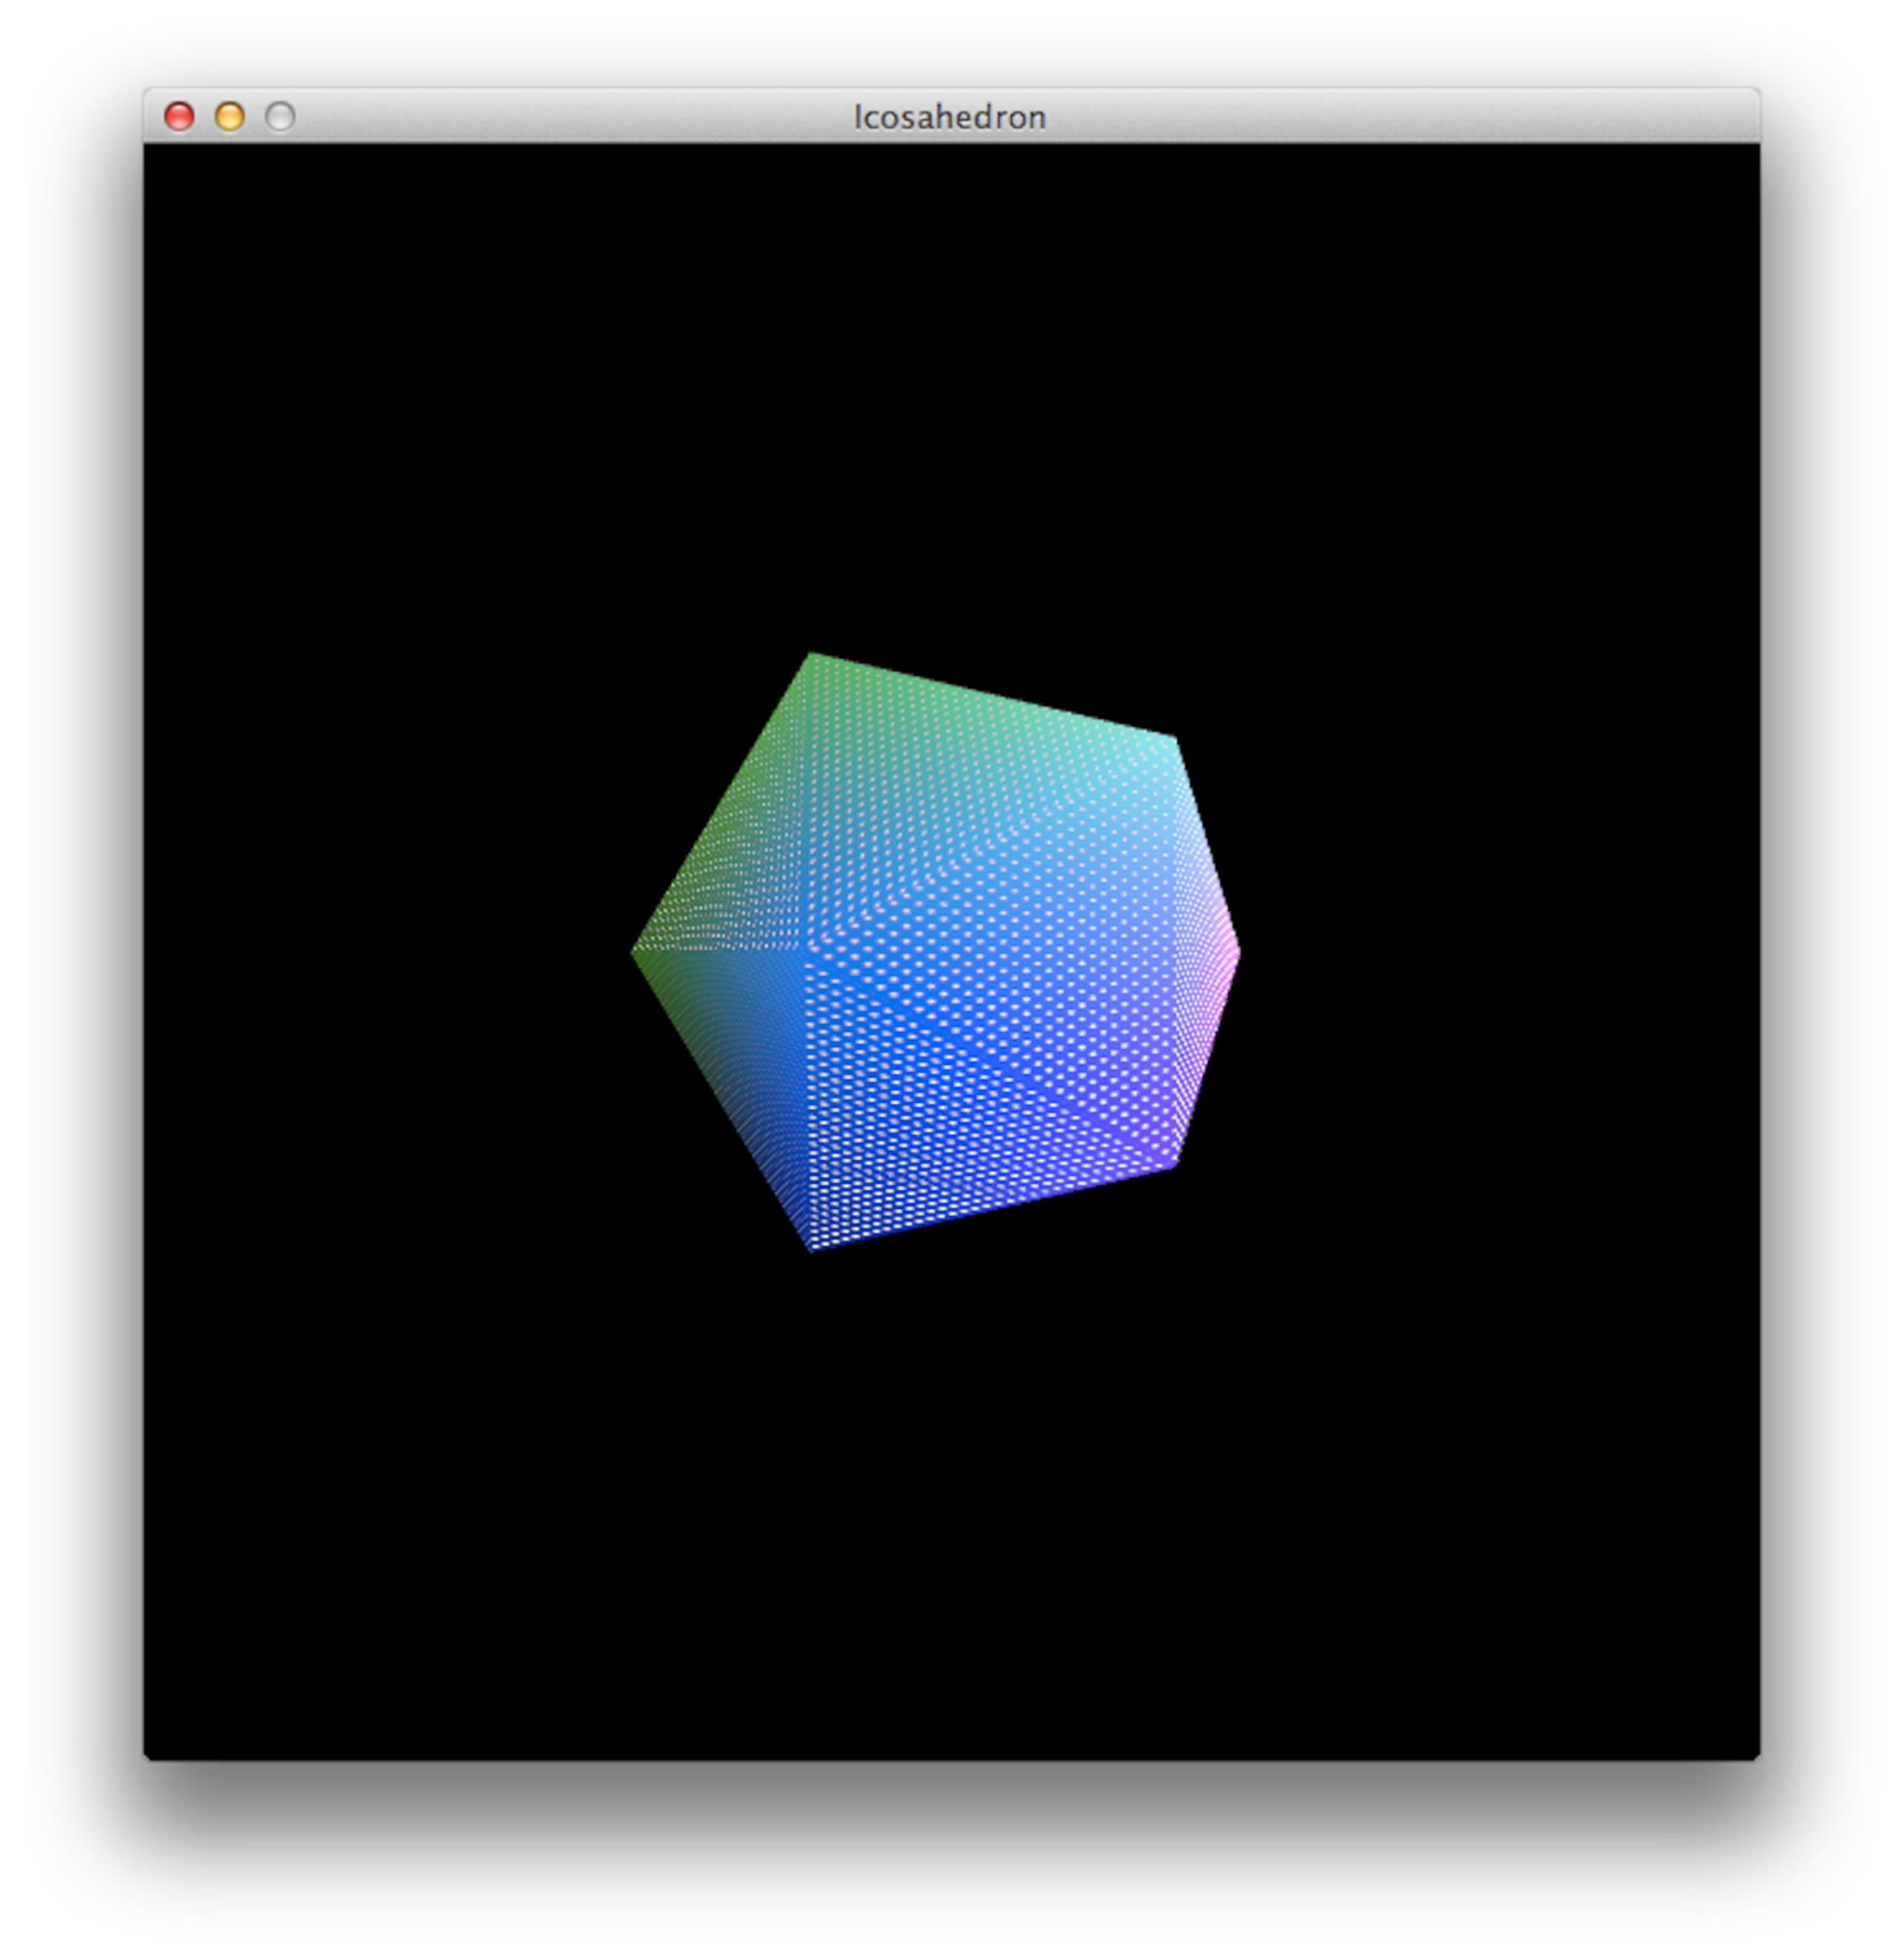
\includegraphics[bb=0 0 444 1200,width=4cm]{Icosahedron_a_and_b.pdf}
\end{figure}
スクリーンショットで示すのは,鏡面反射(光源$L=(0.0,10.0,-10.0)$)と拡散(環境光係数$a=0.5$)の組み合せです.

次の二つの画像に分解できる.
\begin{figure}[H]
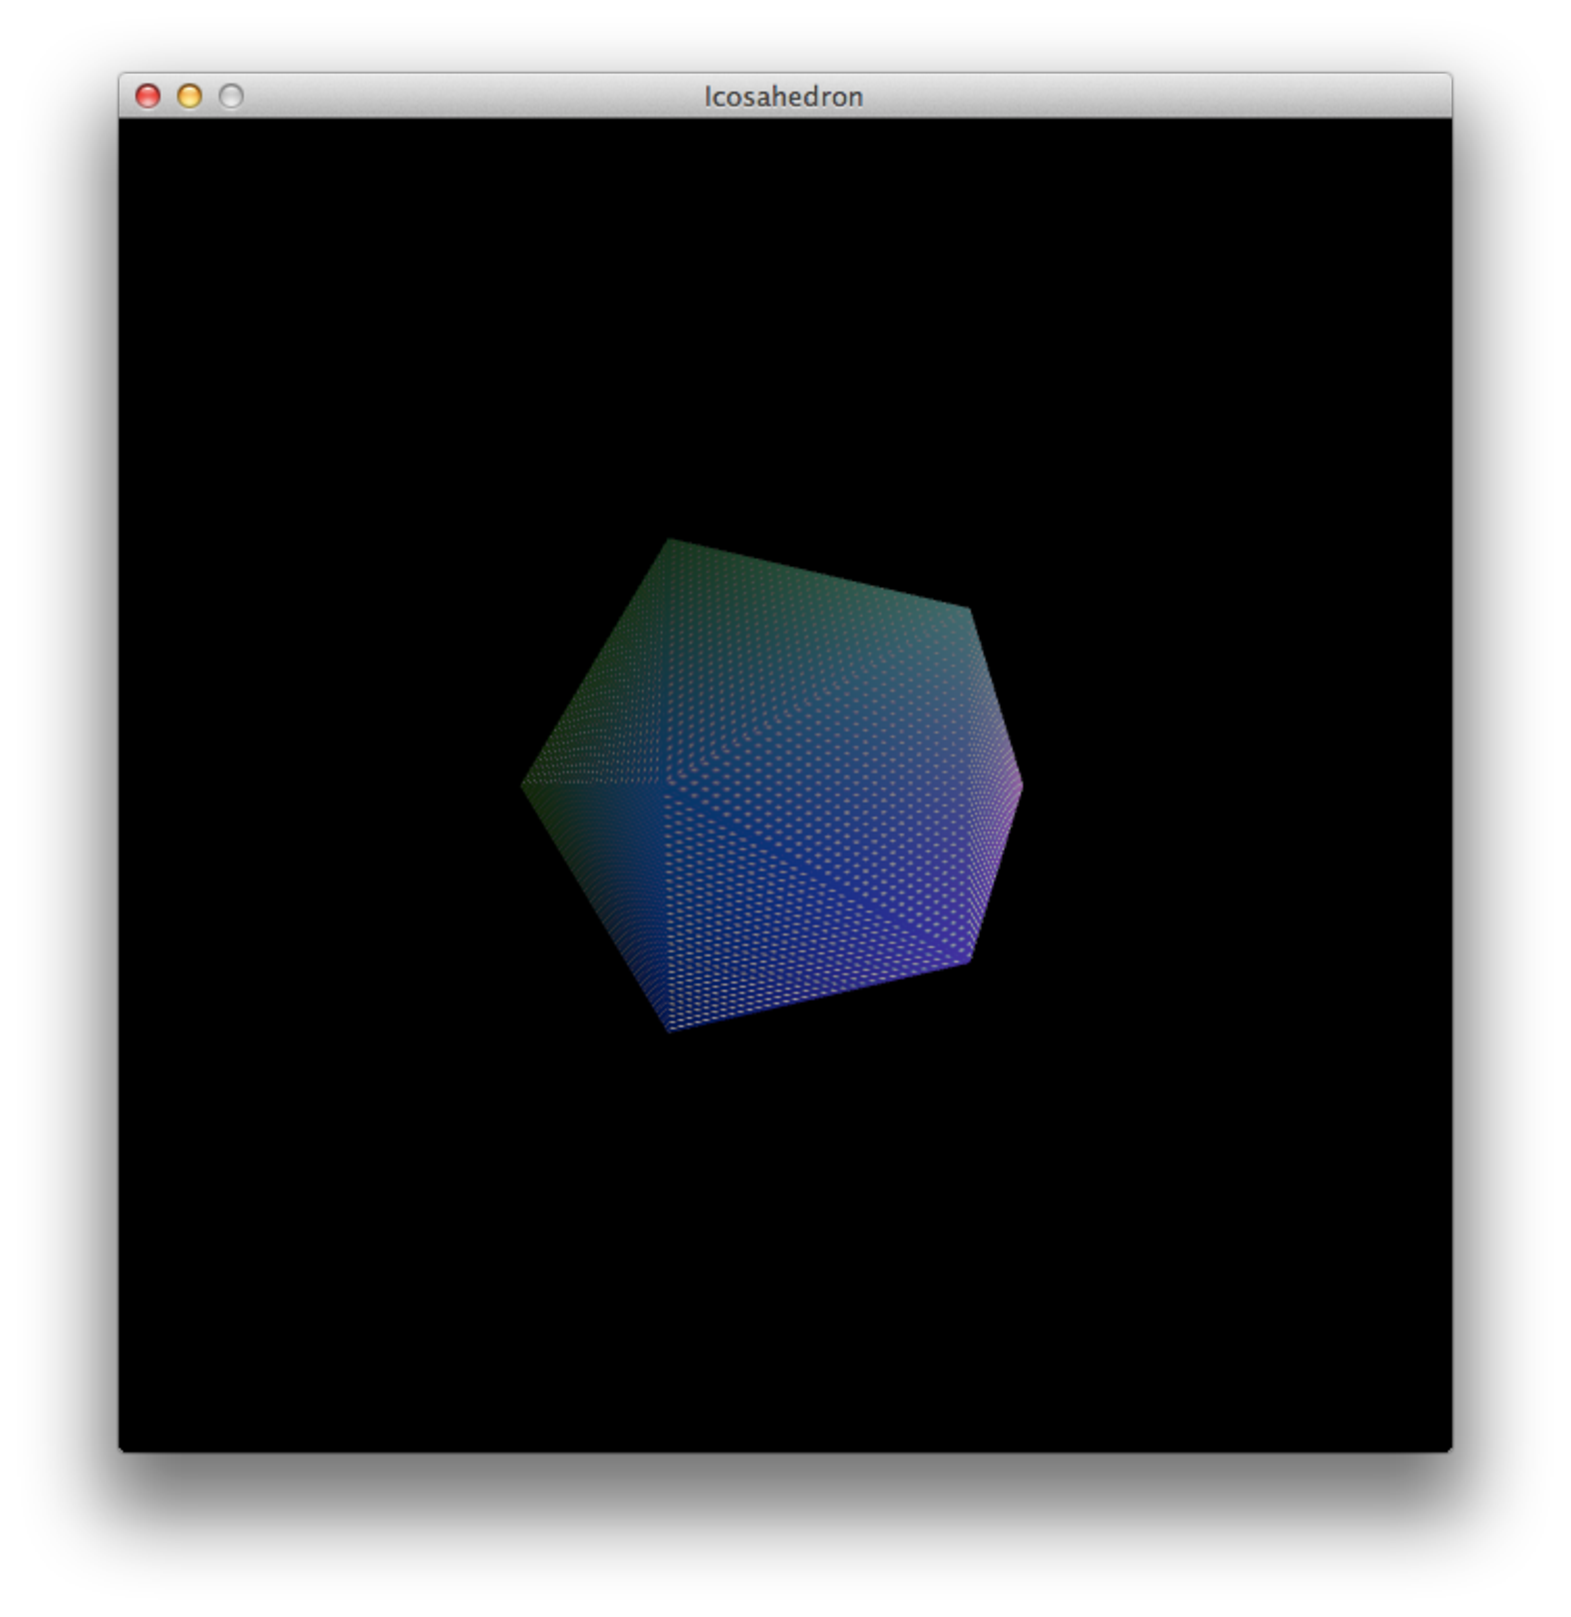
\includegraphics[bb=0 0 444 751,width=6cm]{Icosahedron_a.pdf}鏡面反射
\end{figure}
\begin{figure}[H]
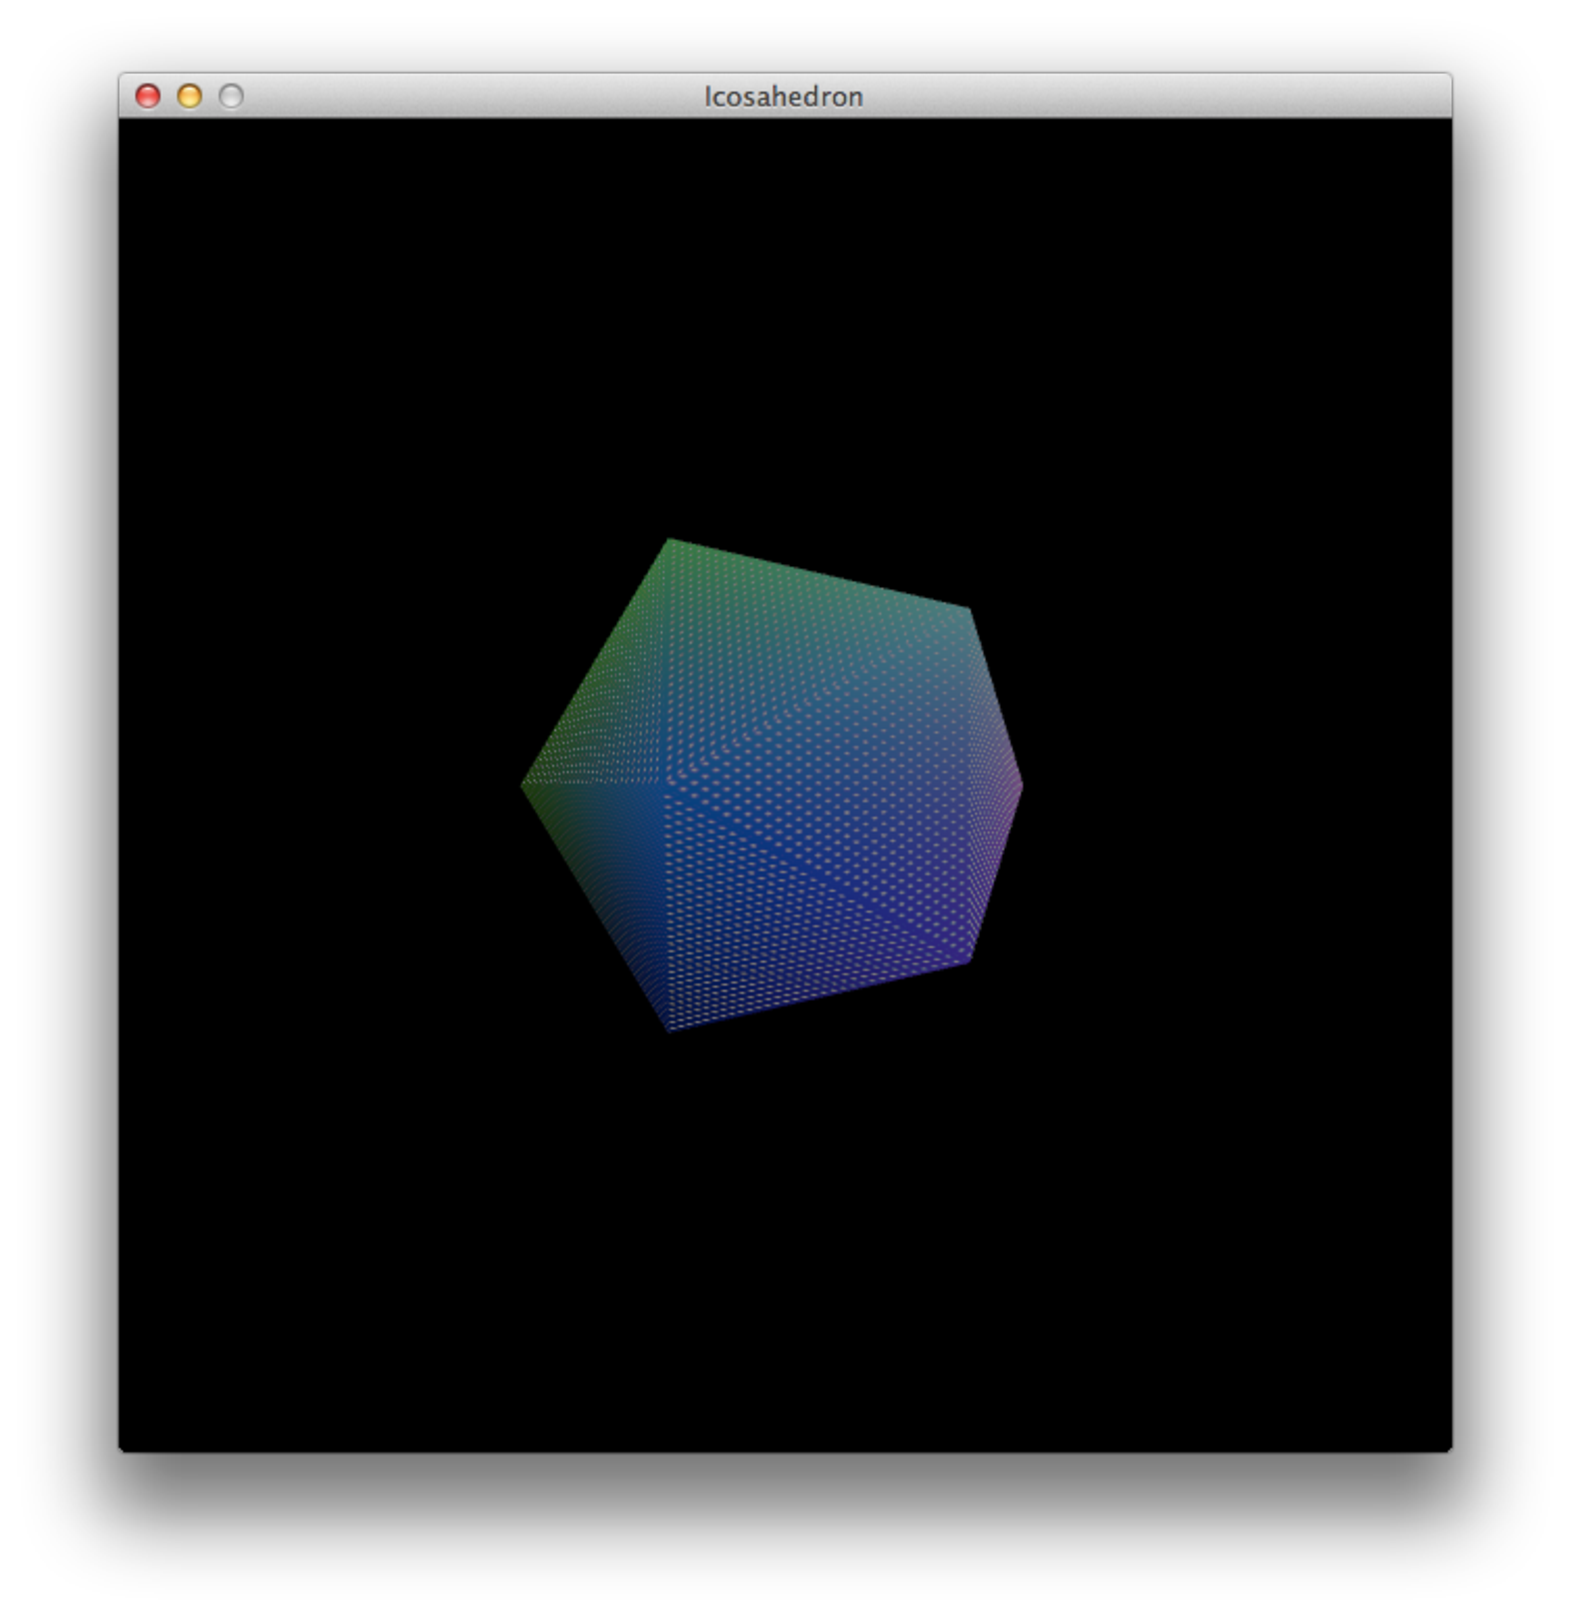
\includegraphics[bb=0 0 444 751,width=6cm]{Icosahedron_b.pdf}拡散
\end{figure}

\end{document}